\documentclass{beamer}
\usepackage[english,russian]{babel}
\usepackage[utf8]{inputenc}
%\usepackage{smaller}
\usepackage{multicol}
\usepackage{tabularx}
\usepackage{wasysym}

%biblatex-gost
\usepackage[backend=biber, style=gost-authoryear, bibstyle=gost-authoryear, language=auto, babel=other, bibencoding=utf8, bibdoi=false, biburl=false,  movenames=false, sortcites = false]{biblatex}
\addbibresource{../txt/sophia_base.bib}


\mode<presentation>
%\mode<article>
% Стиль презентации
%\usetheme{Warsaw}
% \usetheme{Madrid}
\usetheme{Marburg}
%\usetheme{Hannover}
%\usetheme{Singapore}
%\usecolortheme{seahorse}



% в начале каждого раздела печатаем содержание с выделением текущего раздела
%\AtBeginSection[]
%{
%  \begin{frame}<beamer>{Содержание}
%    \tableofcontents[currentsection]
%  \end{frame}
%}




\begin{document}

\title[]{ОРГАНИЗАЦИЯ ПОСЕЛЕНИЙ\\ {\it Macoma~balthica}~(Linnaeus,~1758)\\ В ОСУШНОЙ ЗОНЕ БЕЛОГО И БАРЕНЦЕВА МОРЕЙ}
\author[]{София Александровна Назарова \\ \medskip
	\footnotesize{Научный руководитель: д.б.н.~Н.~В.~Максимович}}
\institute[СПбГУ]{Санкт-Петербургский государственный университет}
\date{Санкт-Петербург, 2015} 

% Создание заглавной страницы
\frame{\titlepage} 



% Автоматическая генерация содержания
%\frame{\frametitle{Содержание}\tableofcontents} 


%%%%%%%%%%%%%%%%%%%%%%%%%%%%%%%%%%%%%%%%%%%%%%%%%%%%%
		\section{Введение}
%%%%%%%%%%%%%%%%%%%%%%%%%%%%%%%%%%%%%%%%%%%%%%%%%%%%%
\begin{frame}{Цели и задачи}
\begin{description}
	\item[Цель.] Изучение организации поселений {\it Macoma balthica} в условиях осушной зоны Белого и Баренцева морей.

	\item[Задачи.]
Для этого были изучены следующие стороны организации поселений:
  \begin{enumerate}
    \item биотический и абиотический фон биотопов;
    \item структурные характеристики поселений \textit{M.~balthica} (показатели обилия, размерная структура);
    \item многолетняя динамика поселений \textit{M.~balthica};
    \item скорость линейного роста моллюсков;
    \item режим формирования спата.
  \end{enumerate}
\end{description}
\end{frame}

%%%%%%%%%%%%%%%%%%%%%%%%%%%%%%%%%%%%%%%%%%%%%%%%%%%%%
		\section[Обилие]{Обилие {\it Macoma balthica}}
%%%%%%%%%%%%%%%%%%%%%%%%%%%%%%%%%%%%%%%%%%%%%%%%%%%%%


\begin{frame}{Обилие {\it M.~balthica} в европейской части ареала}
	\begin{minipage}[t]{.49\linewidth}
		\begin{center}
		{\footnotesize Плотность поселения}
			\includegraphics[width=\textwidth]{Nmean_ru1.pdf}\\[1ex]
%			\includegraphics[width=\textwidth]{lat_vs_Nmean_big1.pdf}\\
%{\small Корреляция Спирмена: $r_{s} = -0,43$, $p < 0,0006$.}
		\end{center}
	\end{minipage}
%
	\begin{minipage}[t]{.49\linewidth}
		\begin{center}
		{\footnotesize Биомасса}
			\includegraphics[width=\textwidth]{Bmean_ru1.pdf}\\[1ex]
%			\includegraphics[width=\textwidth]{lat_vs_Bmean_big1.pdf}\\
%{\small Корреляция Спирмена: $r_{s} = -0,3$, $p < 0,06$.}
		\end{center}
	\end{minipage}

{\tiny Средние значения показателей пропорциональны площади круга на карте}
\end{frame}



%%%%%%%%%%%%%%%%%%%%%%%%%%%%%%%%%%%%%%%%%%%%%%%%%%%%%
		\section[Динамика численности]{Динамика плотности поселений {\it Macoma balthica} в Белом море}
%%%%%%%%%%%%%%%%%%%%%%%%%%%%%%%%%%%%%%%%%%%%%%%%%%%%%

\begin{frame}{Динамика плотности поселений {\it M.~balthica} в вершине Кандалакшского залива}
	\begin{minipage}[b]{.45\linewidth}
		\begin{center}
			\includegraphics[height=.32\textheight]{N2_dynamic_Luvenga_big1.pdf}\\
			\includegraphics[height=.32\textheight]{N2_dynamic_North_big1.pdf}
		\end{center}
{\tiny По оси ординат указана средняя плотность поселения без учета спата}
	\end{minipage}
\hfill
	\begin{minipage}[b]{.5\linewidth}
		\begin{center}
{\scriptsize Синхронность динамики\\ плотности поселений \\в Кандалакшском заливе\\ Белого моря\\}
			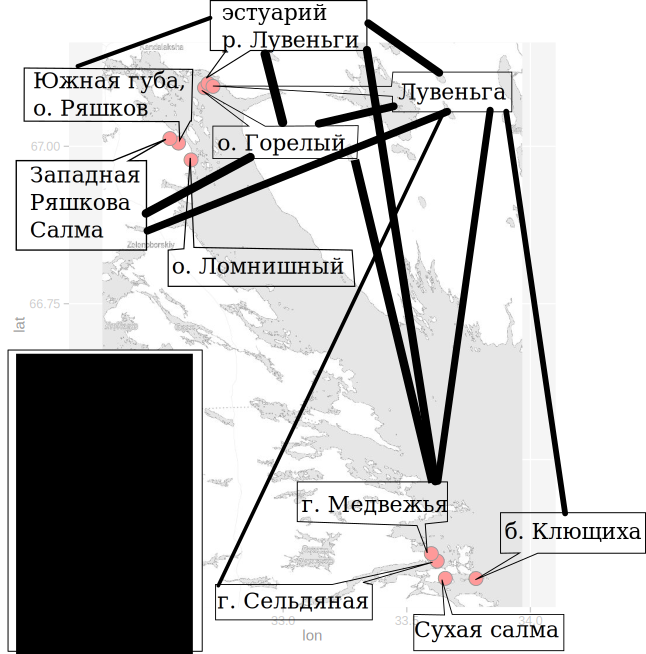
\includegraphics[height=.55\textheight]{mantel_map.pdf}
		\end{center}
	\end{minipage}
\end{frame}

\begin{frame}{Моделирование влияния температуры на численность {\it M.~balthica} в Кандалакшском заливе Белого моря}
$$\ln(N_{t1}) = 1,96 + 0,60 \times \ln(N_{t}) - 0,09 \times T_{wt1}$$
{\scriptsize $F = 37,04$; $p < 0,0001$. $R^2 = 0,6$.} \\
	\begin{minipage}[t]{.49\linewidth}
		\begin{center}
			\includegraphics[width=\textwidth]{./lodNt_vs_logNt1_2.pdf}
		\end{center}
	\end{minipage}
%
	\begin{minipage}[t]{.49\linewidth}
		\begin{center}
			\includegraphics[width=\textwidth]{./Twt1_vs_logNt1_2.pdf}
		\end{center}
	\end{minipage}
{\tiny $\log(N_{t1})$ и $\log(N_{t})$~--- логарифм средней численности маком в данный ($t1$) и предыдущий ($t$) годы; $T_{wt1}$~--- среднезимняя температура в текущий год.}
\end{frame}

%%%%%%%%%%%%%%%%%%%%%%%%%%%%%%%%%%%%%%%%%%%%%%%%%%%%%
		\section[Размерная структура]{Характер размерной структуры поселений {\it Macoma balthica}}
%%%%%%%%%%%%%%%%%%%%%%%%%%%%%%%%%%%%%%%%%%%%%%%%%%%%%

\begin{frame}{Организация поселений {\it M.~balthica}: динамика размерной структуры}
	\begin{minipage}[t]{.53\linewidth}
		\begin{center}
			{\scriptsize Распространение типов динамики размерной структуры в Белом море}\\
			\includegraphics[width=\textwidth]{map_size_distr.pdf}\\
\textcolor{red}{\scriptsize +поселение в г.~Дальне-Зенеленцкой Баренцева моря}
		\end{center}

	\end{minipage}
%
	\begin{minipage}[t]{.45\linewidth}
		\begin{center}
	\textcolor{red}{\footnotesize Чередование вариантов\\ размерной структуры}
			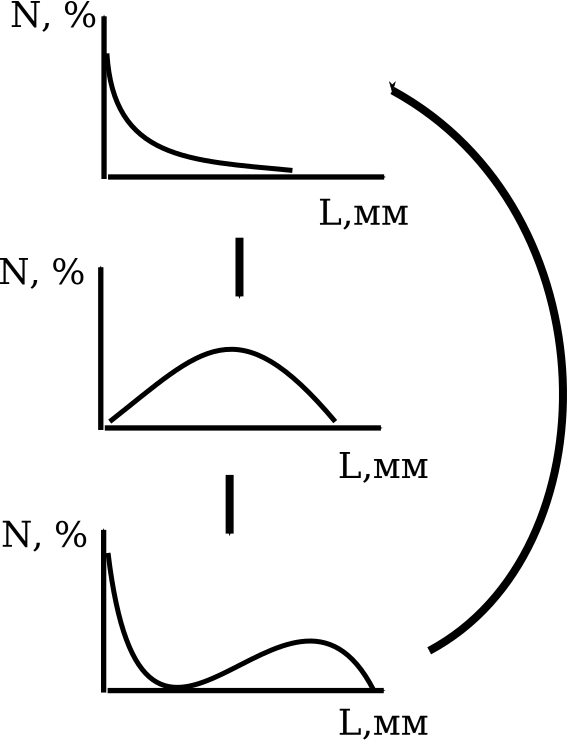
\includegraphics[width=.65\textwidth]{Dymanic_cheredovanie.pdf}

	\textcolor{blue}{\footnotesize Ежегодное повторение\\ размерной структуры}\\
			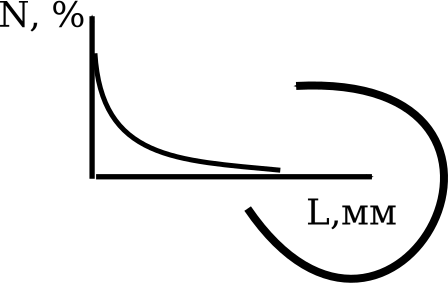
\includegraphics[width=.65\textwidth]{Dymanic_povtorenie.pdf}\\


		\end{center}
	\end{minipage}
\end{frame}

%%%%%%%%%%%%%%%%%%%%%%%%%%%%%%%%%%%%%%%%%%%%%%%%%%%%%
		\section[Линейный рост]{Линейный рост {\it Macoma balthica}}
%%%%%%%%%%%%%%%%%%%%%%%%%%%%%%%%%%%%%%%%%%%%%%%%%%%%%
\begin{frame}{Линейный рост {\it M.~balthica} в европейской части ареала}
	\begin{minipage}[t]{.52\linewidth}
		\begin{center}
			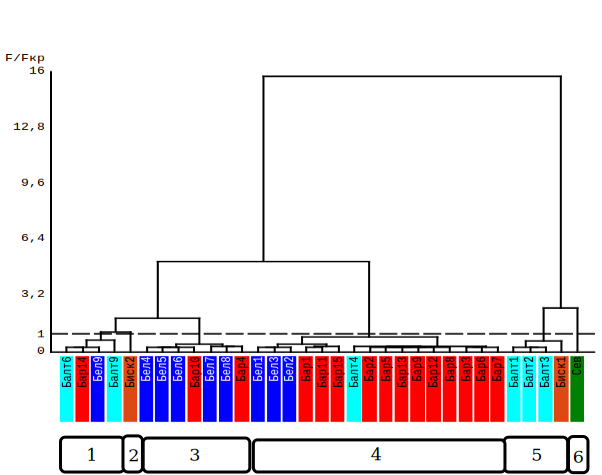
\includegraphics[width=\textwidth]{./Europe_clusters_usrednenie.pdf}
		\end{center}

Цветовые обозначения: \textcolor{red}{Баренцево море}, 
\textcolor{blue}{Белое море}, 
\textcolor{cyan}{Балтийское море}, 
\textcolor{green}{Северное море}, 
\textcolor{brown}{Бискайский залив}.
	\end{minipage}
%
	\begin{minipage}[t]{.45\linewidth}
		\begin{center}
			\includegraphics[width=\textwidth]{./Europe_growth_groups_prizm.pdf}
		\end{center}
	\end{minipage}
\end{frame}

%%%%%%%%%%%%%%%%%%%%%%%%%%%%%%%%%%%%%%%%%%%%%%%%%%%%%
		\section[Оседание]{Режим формирования спата}
%%%%%%%%%%%%%%%%%%%%%%%%%%%%%%%%%%%%%%%%%%%%%%%%%%%%%
\begin{frame}{Обилие спата \textit{Macoma balthica}}
		\begin{center}
			\includegraphics[width=\textwidth]{N_spat1.pdf}
		\end{center}
\end{frame}



%%%%%%%%%%%%%%%%%%%%%%%%%%%%%%%%%%%%%%%%%%%%%%%%%%%%%
		\section{Выводы}
%%%%%%%%%%%%%%%%%%%%%%%%%%%%%%%%%%%%%%%%%%%%%%%%%%%%%
\begin{small}

\begin{frame}{Выводы}
\addtocounter{enumi}{0}
	\begin{enumerate}
		\item В Кольском заливе Баренцева моря и Кандалакшском заливе  Белого моря значения биомассы (до 200 г/м$^2$) поселений {\it Macoma balthica} сопоставимы с аналогичным показателем в европейской части ареала, а плотность поселений нередко оказывается выше (до 8~тыс.~экз./м$^2$). Для литорали восточной части Мурманского побережья Баренцева моря типичны поселения {\it M.~balthica} с численностью менее 100 экз./м2 
		\item Плотность поселений спата {\it Macoma balthica} в Белом море может варьировать на порядок в пределах незначительной акватории, и достигать десятков тысяч экз./м$^2$.
		\item Беломорские и баренцевоморские поселения {\it M.~balthica} не различаются по средней скорости роста моллюсков, и отличаются по этому показателю минимальными характеристиками в пределах европейской части ареала вида. 
	\end{enumerate}
\end{frame}


\begin{frame}{Выводы}
	\begin{enumerate}
\addtocounter{enumi}{3}
		\item Динамика размерной структуры поселений {\it Macoma balthica} в Белом и Баренцевом представлена двумя типами. \\
Наболее обычный вариант~--- чередование бимодального и мономодального распределений особей по размерам. При этом первый пик формируют молодые
особи (обычно длиной до 5 мм), а второй модальный класс состоит из взрослых особей (в Белом море длиной 9--12~мм, в Баренцевом море~--- 10--17~мм).
Как относительно редкое событие наблюдается мономодальная структура поселений с ежегодным преобладаем молоди.
		\item Динамика плотности поселений {\it Macoma balthica} в Кандалакшском заливе Белого моря демонстрирует элементы синхронности в поселениях, расположенных на расстоянии от 1 до 100~км, что происходит на фоне резкой межгодовой неравномерности пополнения поселений молодью.  
	\end{enumerate}
\end{frame}


\end{small}

\end{document}

